% Chapter Template

\chapter{Experimentation} % Main chapter title

\label{Experimentation} % Change X to a consecutive number; for referencing this chapter elsewhere, use \ref{ChapterX}

\section{Model Hyperparameters}

\subsection{Compute Resources}

The model was mainly trained on a single \textbf{NVIDIA GeForce 3090} GPU, which is currently one of the highest end graphics cards. However, this GPU is significantly more compute power than is needed in order to train the model. The GPU used to train this model has 24 GB memory, whereas the model typically only takes ~3.5 GB GPU memory at max. This would in theory mean the model could be trained on less current, and cheaper hardware such as the \textbf{NVIDIA GeForce GTX-1660}. The model is also almost certainly compact enough to be trained on purely CPU, however this would of course result in large training time increases.

\section{JHMDB Results}

The dataset that the model will be evaluated on will be the JHMDB dataset. As previously stated in section \ref{sec:datasets}, JHMDB is a good dataset to evaluate performance on pose-based models. The dataset contains 3 splits, each of which have a training and testing pair. Three independent models will be trained, one on each of the splits, without any previous pre-training, and with randomly initialized weights that will be seeded such that they're consistent from one run to another.

\begin{table}[ht]
	\centering
	\begin{tabular}{||c c||} 
		\hline
		\textbf{Split} & \textbf{Accuracy} \\ [0.5ex] 
		\hline\hline
		1 & 58.209\% \\ 
		\hline
		2 & 58.889\% \\
		\hline
		3 & 58.113\% \\
		\hline
		\hline
		\textbf{Average} & \textbf{58.404\%} \\
		\hline
	\end{tabular}
	\caption{Results on all 3 splits of the JHMDB dataset utilizing only our novel approach.}
	\label{tab:acc-results}
\end{table}

Table \ref{tab:acc-results} contains the accuracy results of the previously discussed model and representation on the JHMDB dataset. As can be seen the model obtains on average a 58\% testing accuracy using only the novel approach presented. This is a sufficient accuracy to show that action recognition is possible with very lightweight representations that can then be processed via smaller models that can be run on less advanced hardware.

These accurate results do not tell the complete story however. As can be seen from the individual class F1 scores in figure \ref{fig:detailed-f1}, some classes the model is fairly good at predicting classes that have very clear movements associated with them such as $golf$, $pullup$, or $swing\_baseball$. The significance of these classes is that the variance of the movement from one person to another is not very significant, so the model is able to learn the joint movements and apply that logic to other classes.

\begin{figure}[ht]
	\includegraphics[width=10cm]{detailedF1}
	\centering
	\caption{Detailed F1 score results on the JHMDB dataset, averaged over the 3 testing splits. Black bars show the corresponding maximum \& minimum values attained in one of the splits.}
	\label{fig:detailed-f1}
\end{figure}

The opposite factor is also something to consider. Figure \ref{fig:jump-comparison} shows an example of three different sets of frames from the $jump$ class. As can be seen from the frames, there are many different ways that a person may perform the $jump$ action. A good example is the final two frames from figure \ref{fig:jump-comparison-a}, where the person simply moves throughout the global position of the frame, rather than actually moving any of their joints. Comparing to figures \ref{fig:jump-comparison-b} or \ref{fig:jump-comparison-c}, where there are many joint movements throughout the frames, makes it difficult for the model to interpret them as the same and generalize to other examples of the same class. Figures \ref{fig:jump-comparison-b} and \ref{fig:jump-comparison-c} also demonstrate the variability in how these actions can be performed when they are general, where \ref{fig:jump-comparison-b} shows more of a twisting motion, \ref{fig:jump-comparison-c} is a more typical "jump".

\begin{figure}[ht]
	\subfigure[]{
		\includegraphics[width=3cm]{JumpFrames/A/00001.png}
		\includegraphics[width=3cm]{JumpFrames/A/00005.png}
		\includegraphics[width=3cm]{JumpFrames/A/00010.png}
		\includegraphics[width=3cm]{JumpFrames/A/00015.png}
		\label{fig:jump-comparison-a}
	}
	\subfigure[]{
		\includegraphics[width=3cm]{JumpFrames/B/00001.png}
		\includegraphics[width=3cm]{JumpFrames/B/00005.png}
		\includegraphics[width=3cm]{JumpFrames/B/00010.png}
		\includegraphics[width=3cm]{JumpFrames/B/00015.png}
		\label{fig:jump-comparison-b}
	}
	\subfigure[]{
		\includegraphics[width=3cm]{JumpFrames/C/00001.png}
		\includegraphics[width=3cm]{JumpFrames/C/00010.png}
		\includegraphics[width=3cm]{JumpFrames/C/00020.png}
		\includegraphics[width=3cm]{JumpFrames/C/00030.png}
		\label{fig:jump-comparison-c}
	}
	\centering
	\caption{Three examples of the $Jump$ class from the JHMDB dataset. The frames selected were four frames roughly evenly spaced out through the video.}
	\label{fig:jump-comparison}
\end{figure}

This low variability in the $golf$ class can also be demonstrated in a similar fashion to this. Figure \ref{fig:golf-comparison} demonstrates this behaviour, where the action is nearly always performed in the same way where a person is standing, reaches back, twists and pulls the club forwards. Figures \ref{fig:golf-comparison-a} and \ref{fig:golf-comparison-c} are perhaps the best examples as they are swinging similar clubs, so the way that they move is almost identical, therefore meaning that the intermediate representation will also be similar. Figure \ref{fig:golf-comparison-b} is again a very similar movement, however it is a slightly different club meaning the movement is not as pronounced. 

\begin{figure}[ht]
	\subfigure[]{
		\includegraphics[width=3cm]{GolfFrames/A/00001.png}
		\includegraphics[width=3cm]{GolfFrames/A/00010.png}
		\includegraphics[width=3cm]{GolfFrames/A/00020.png}
		\includegraphics[width=3cm]{GolfFrames/A/00030.png}
		\label{fig:golf-comparison-a}
	}
	\subfigure[]{
		\includegraphics[width=3cm]{GolfFrames/B/00001.png}
		\includegraphics[width=3cm]{GolfFrames/B/00005.png}
		\includegraphics[width=3cm]{GolfFrames/B/00010.png}
		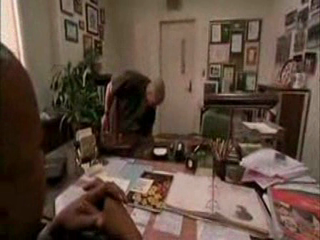
\includegraphics[width=3cm]{GolfFrames/B/00023.png}
		\label{fig:golf-comparison-b}
	}
	\subfigure[]{
		\includegraphics[width=3cm]{GolfFrames/C/00001.png}
		\includegraphics[width=3cm]{GolfFrames/C/00010.png}
		\includegraphics[width=3cm]{GolfFrames/C/00020.png}
		\includegraphics[width=3cm]{GolfFrames/C/00030.png}
		\label{fig:golf-comparison-c}
	}
	\centering
	\caption{Three examples of the $Golf$ class from the JHMDB dataset. The frames selected were four frames roughly evenly spaced out through the video.}
	\label{fig:golf-comparison}
\end{figure}

The detailed precision and recall values broken down by class are shown in figures \ref{fig:detailed-precision} and \ref{fig:detailed-recall}, and in general reflect the same results as the F1 scores. The only notable difference is the model tends to have higher recall differences and precision tends to be closer from one class to another.

\begin{figure}[ht]
	\includegraphics[width=10cm]{detailedPrecision}
	\centering
	\caption{Detailed precision results on the JHMDB dataset, averaged over the 3 testing splits. Black bars show the corresponding maximum \& minimum values attained in one of the splits.}
	\label{fig:detailed-precision}
\end{figure}

\begin{figure}[ht]
	\includegraphics[width=10cm]{detailedRecall}
	\centering
	\caption{Detailed recall results on the JHMDB dataset, averaged over the 3 testing splits. Black bars show the corresponding maximum \& minimum values attained in one of the splits.}
	\label{fig:detailed-recall}
\end{figure}

\section{Model Ablation Study}

This section will present both different intermediate representation formats, as well as different model architectures. The natural first step to determining how effective the chosen architecture compared to others is to isolate each of the two halves (angle velocities \& angles themselves). These results are presented in tables \ref{tab:acc-results-v-velocity} and \ref{tab:acc-results-v-angle}.

\begin{table}[ht]
	\centering
	\begin{tabular}{||c c c||} 
		\hline
		\textbf{Split} & \textbf{Stacked} & \textbf{Only Angle Velocity} \\ [0.5ex] 
		\hline\hline
		1 & \textbf{58.209\%} & 48.888\% \\ 
		\hline
		2 & \textbf{58.889\%} & 44.444\% \\
		\hline
		3 & \textbf{58.113\%} & 41.132\% \\
		\hline
		\hline
		\textbf{Average} & \textbf{58.404\%} & 44.821\% \\
		\hline
	\end{tabular}
	\caption{Comparison of results using only angle velocities vs the stacked representation.}
	\label{tab:acc-results-v-velocity}
\end{table}

The only angle velocity results show an average decrease in performance over all three splits of approximately 14\% over the combination of the two. This is a very large decrease in accuracy, but is far from a negative result. What this result shows is that for some classes, the actual movement of the joint can be used in place of the joint angles and it is not necessarily required to have both in the representation. This is shown in figure \ref{fig:detailed-f1-only-change}, where we see that classes such as golf \& pullup still have a relatively high F1-Score of 0.7 on average.

\begin{figure}[ht]
	\includegraphics[width=10cm]{detailedF1OnlyChange}
	\centering
	\caption{Detailed F1 score results on the JHMDB dataset using only the angle velocities from one frame to another.}
	\label{fig:detailed-f1-only-change}
\end{figure}

\begin{table}[ht]
	\centering
	\begin{tabular}{||c c c||} 
		\hline
		\textbf{Split} & \textbf{Stacked} & \textbf{Only Angles} \\ [0.5ex] 
		\hline\hline
		1 & \textbf{58.209\%} & 56.343\% \\ 
		\hline
		2 & \textbf{58.889\%} & \textbf{58.889\%} \\
		\hline
		3 & \textbf{58.113\%} & 56.604\% \\
		\hline
		\hline
		\textbf{Average} & \textbf{58.404\%} & 57.279\% \\
		\hline
	\end{tabular}
	\caption{Comparison of results using only angles vs the stacked representation.}
	\label{tab:acc-results-v-angle}
\end{table}

Similarly, the representation that uses only angles and ignores the angle velocities shows a decrease in performance. However this is much less pronounced, and is only around 1\%. This suggests that while the angle velocities do add value, it is not uniformly a large positive. However when considering how small the actual data still is in the stacked representation the small increase in accuracy is justified.

\section{Model Comparison}